\documentclass{hswbeamer}

\title[EiP]{Einführung in die Programmierung}
\subtitle[WS 2014/15]{Wintersemester 2014/15}
\author[\Copyright{Uwe L\"{a}mmel, Thomas Jonitz}]{Prof. Dr.-Ing Uwe L\"{a}mmel \and Thomas Jonitz (B.Sc.)}
\date{Wismar, 14. Februar 2015}
%\logo{\includegraphics[height=1cm]{fischer.png}}
\titlegraphic{
\includegraphics[scale=0.05]{img/hsw-wings.jpg}}

\bibliography{literatur}
\makeindex
\begin{document}



\begin{frame}
    \begin{quote}
        \glqq Saying Java is nice, because it works on all OSes ist like saying anal sex is nice, because it works on all genders.\grqq -- Icematix (c-plusplus.de)
    \end{quote}
\end{frame}

\begin{frame}
    \maketitle
\end{frame}

\begin{frame}[shrink]{Tagesplanung}
    \begin{block}{Agenda für den Tag}
        \begin{enumerate}
        \item Vorstellungsrunde
        \item Bauplan-Klassen
        \item Arrays und ArrayLists
        \item Keller (Stack) und Schlange (Queue)
        \item Rekursion (Binär-Baum)
        \item Such- und Sortieralgorithmen
        \item Vererbung (Bsp.: Kalender)
        \item Prüfung und Evaluierung
        \end{enumerate}
    \end{block}
    \begin{block}{Vorschlag:}
        \begin{description}
        \item[\Uhr{10}{30}--\Uhr{10}{45}] Frühstückspause
        \item[\Uhr{12}{15}--\Uhr{13}{15}] Mittagspause
        \item[\Uhr{15}{40}--\Uhr{15}{55}] Erfrischung und Vorbereitung
        \end{description}
    \end{block}
\end{frame}

%\section{Vorstellungsrunde}
\begin{frame}[shrink]{Thomas Jonitz}{t.jonitz@wings.hs-wismar.de}
    %\begin{columns}
        %\begin{column}{0.3\textwidth}
            %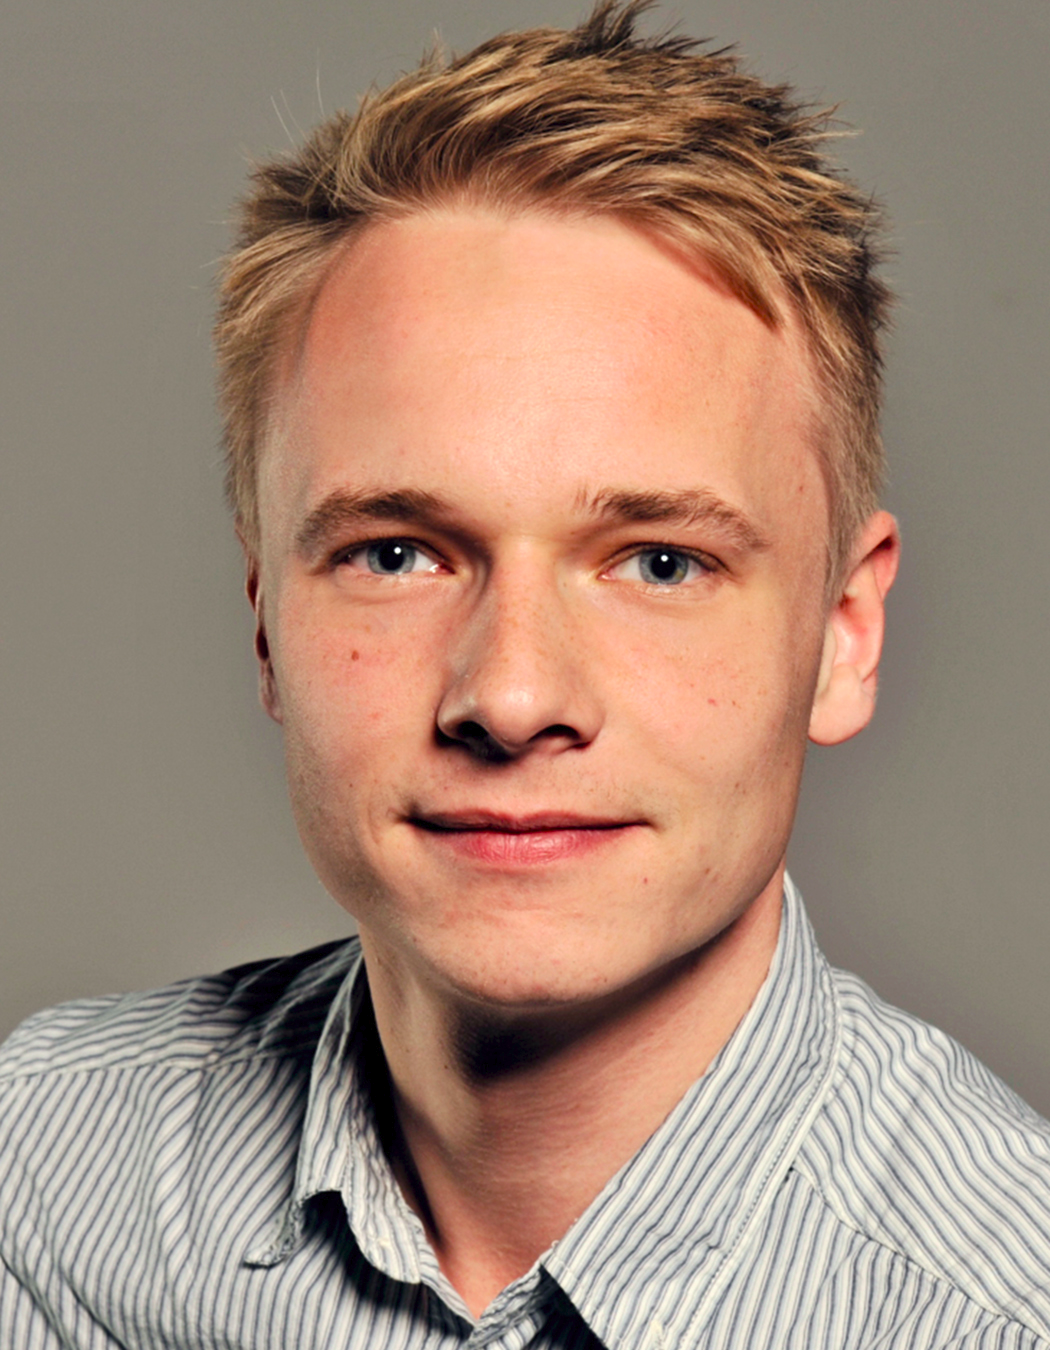
\includegraphics[width=0.6\columnwidth]{img/jonitz.png}
        %\end{column}
        %\begin{column}{0.7\textwidth}
            \begin{block}{Ausbildung}
                \begin{description}
                \item[2007-2009] Industrietechnologe f. Datentechnik
                \item[2009-2013] Wirtschaftsinformatik B.Sc.
                \item[seit 2013] Wirtschaftsinformatik M.Sc.
                \end{description}
            \end{block}
            \begin{block}{Praxis}
                \begin{description}
                \item[2007-2009] Siemens Enterprise Communications
                \item[2011-2013] Softwareentwickler, IAIB e.V.
                \item[2010-2014] Tutor EiP, EWI, AWP
                \item[seit 2014] IT-Beauftragter, WINGS -- Fernstudium GmbH
                \item[seit 2014] Lehrbeauftragter/Dozent EiP
                \end{description}
            \end{block}
        %\end{column}
    %\end{columns}
\end{frame}

%\section{Datensammlungen}
\begin{frame}[shrink]{Hinweis}
\begin{block}{Zur Prüfung}
    Die Prüfung dauert höchstens 120 Minuten.\\
    Es sind keine Hilfsmittel zugelassen.\\
    Sie dürfen eigenes Papier verwenden.\\
    Kommentieren Sie bitte Ihren Quelltext.
\end{block}
\begin{block}{Zur Evaluation}
    Die Evaluation findet anonym statt und wird elektronisch verarbeitet.\\
    Nutzen Sie bitte keine hellen Stifte (Bleistifte, gelbe Stifte etc.)\\
    Wer zuletzt abgibt, muss den Umschlag versiegeln.
\end{block}
\end{frame}

\begin{frame}{}
\end{frame}


\end{document}
